% !TEX root = ../report.tex
\section*{The Experiments} \label{sec:experiments}
\addcontentsline{toc}{section}{The Experiments}

Screenshots of the Push Throw technique demo is shown in \Cref{fig:demovideo}.

\begin{figure}[H]
\subfloat[]{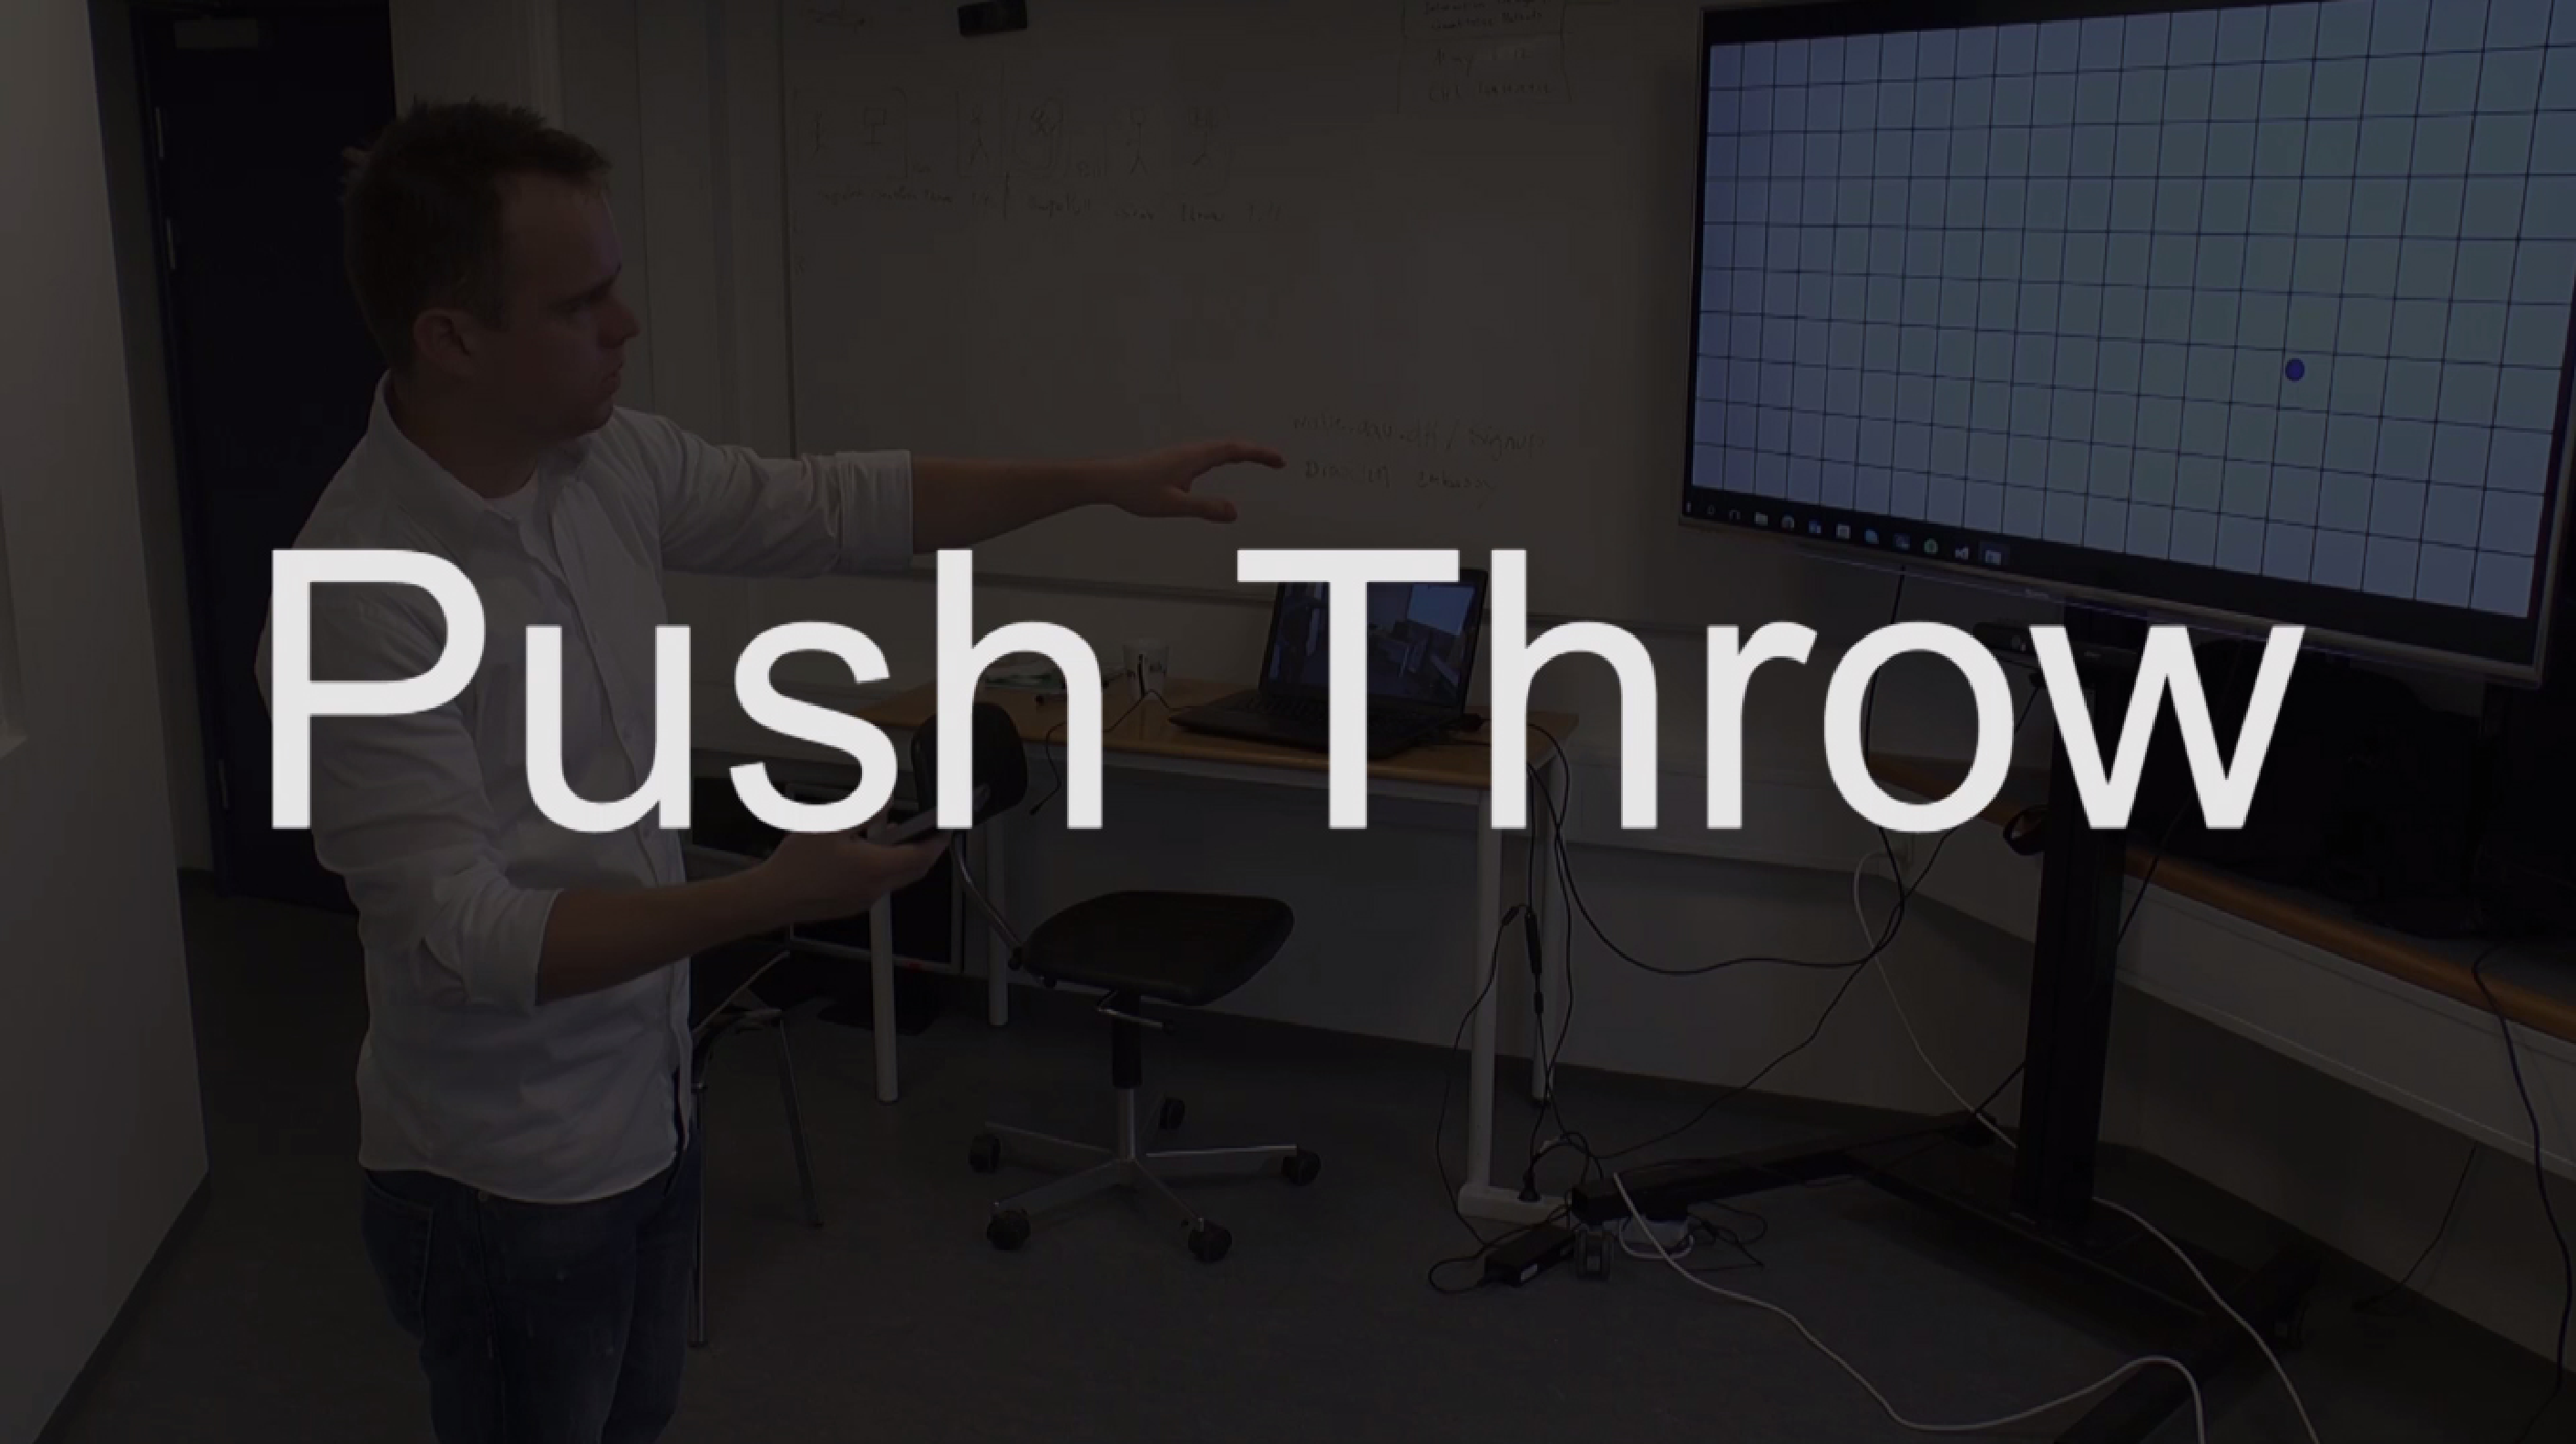
\includegraphics[width = 0.5\columnwidth]{images/demovideo1.pdf}\label{fig:demovideA}}
\subfloat[]{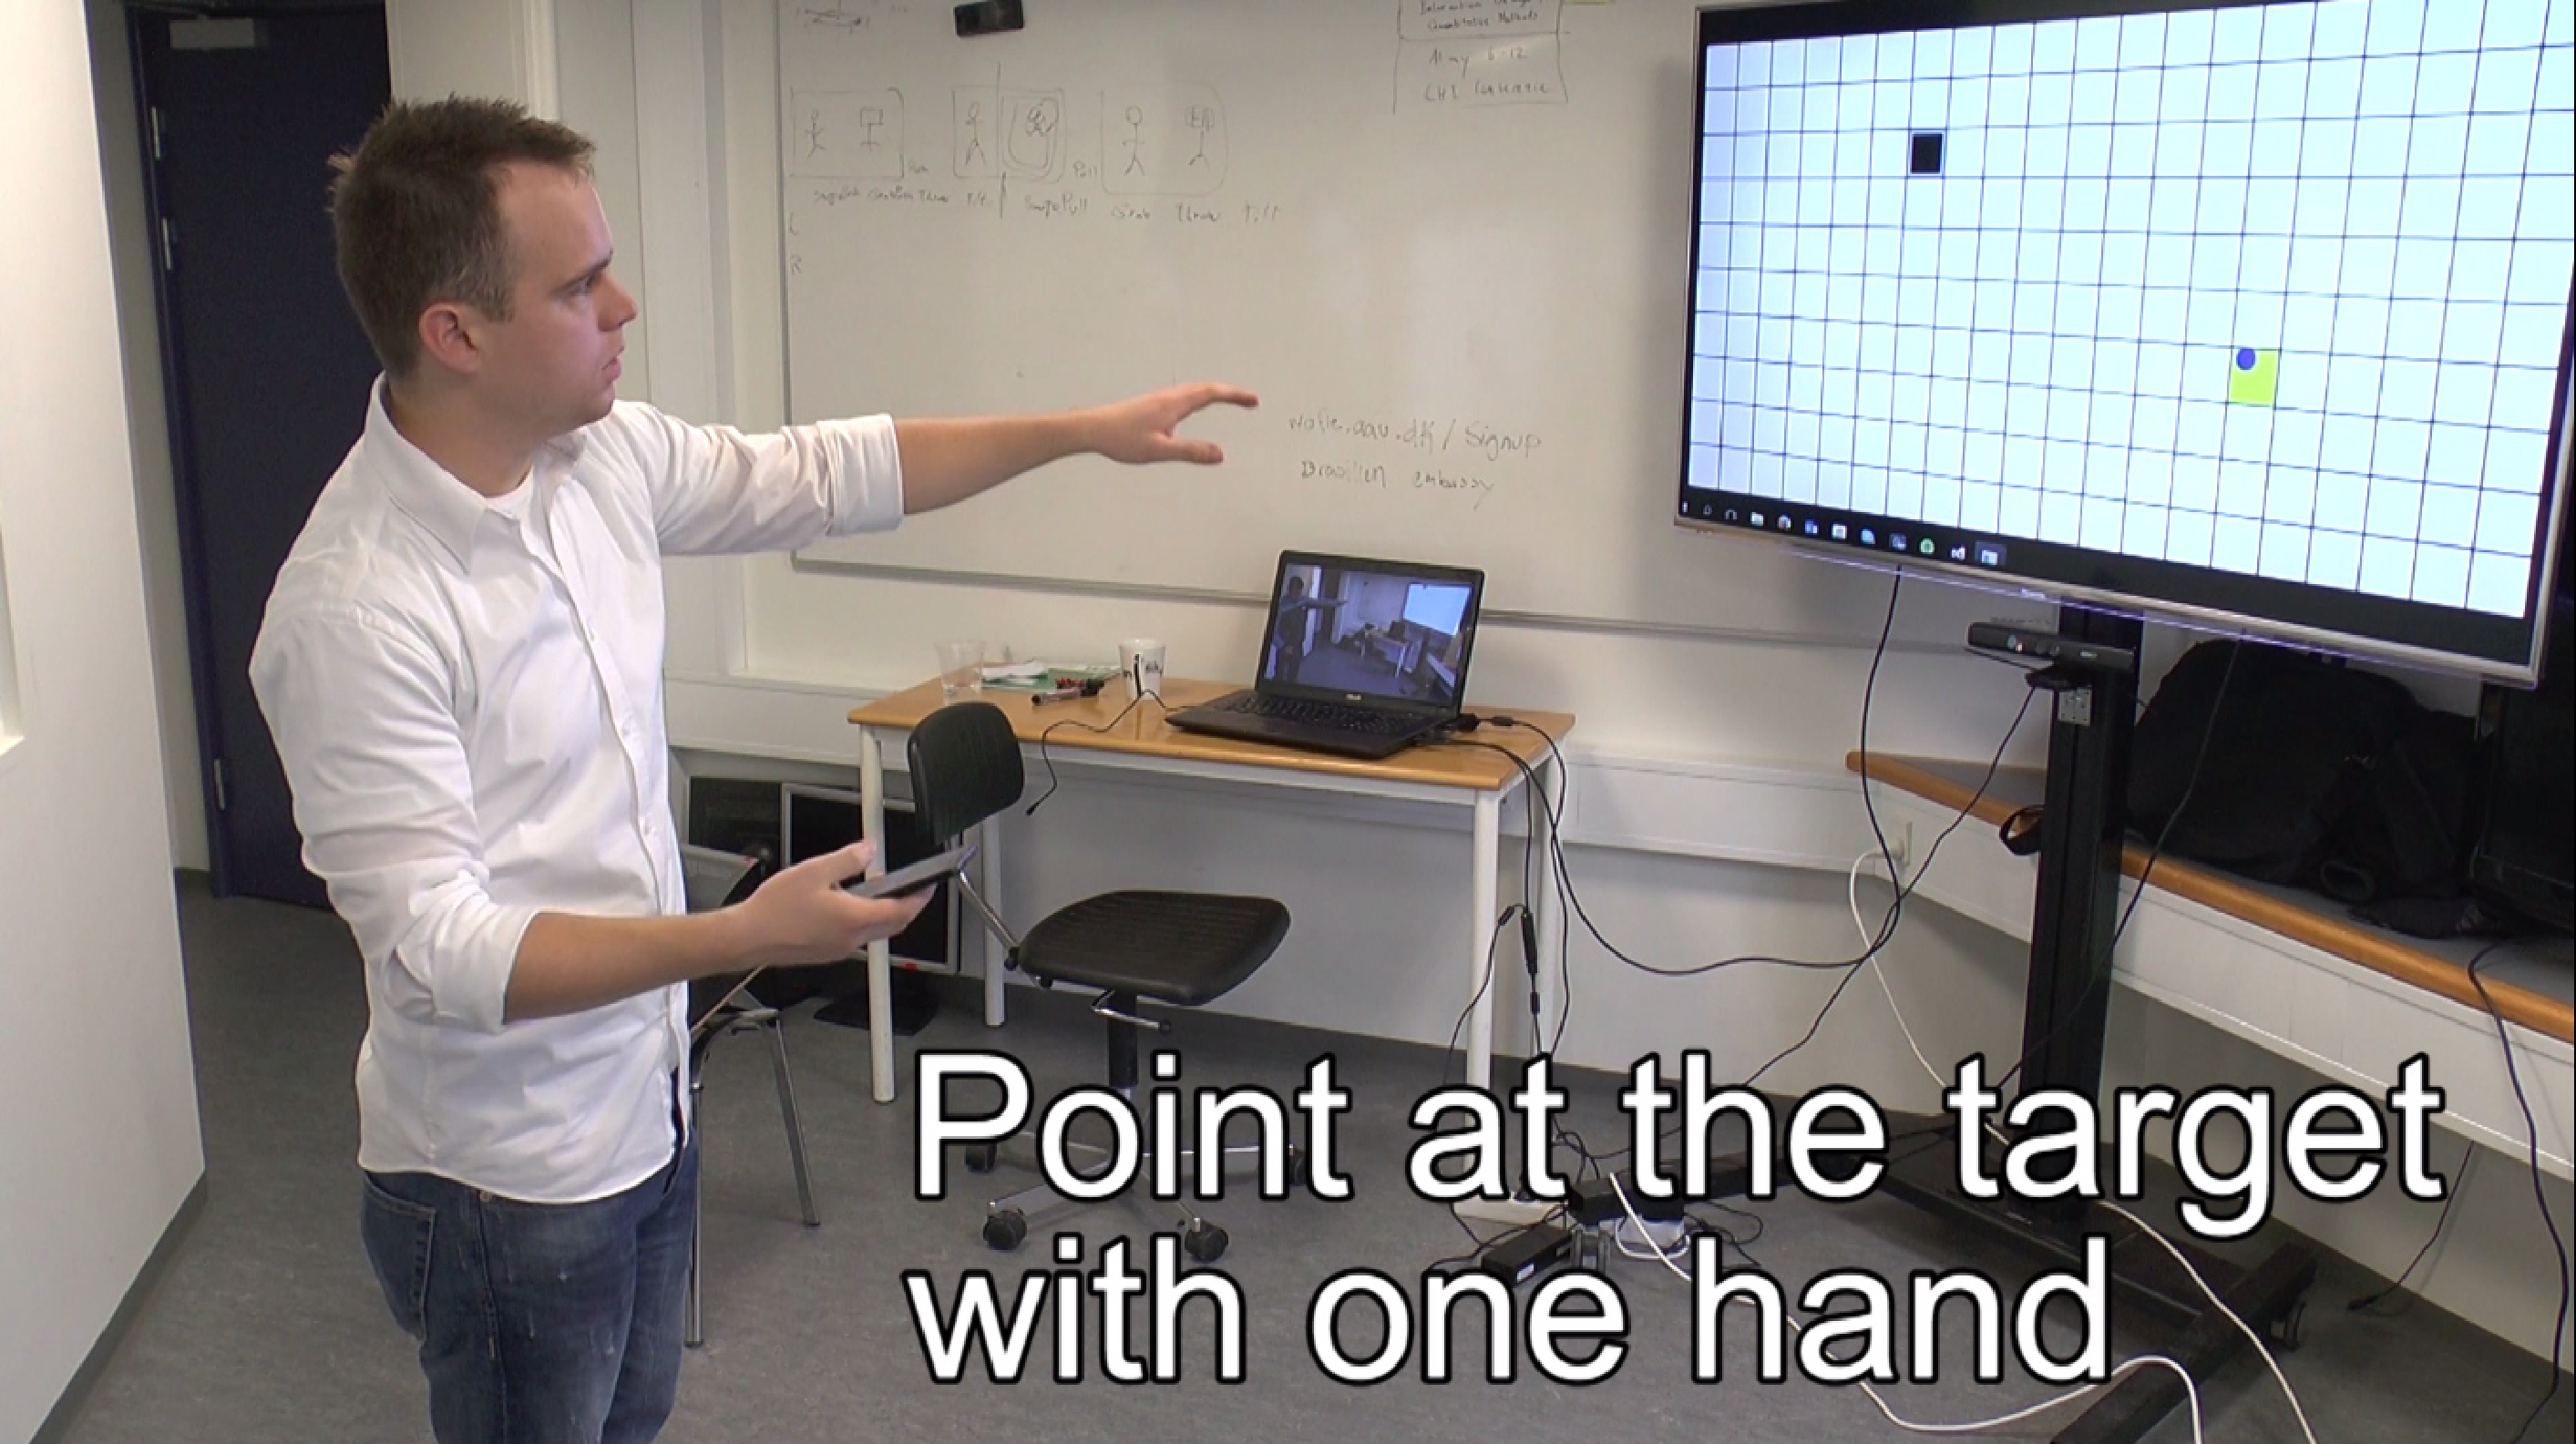
\includegraphics[width = 0.5\columnwidth]{images/demovideo2.pdf}\label{fig:demovideB}}\\
\subfloat[]{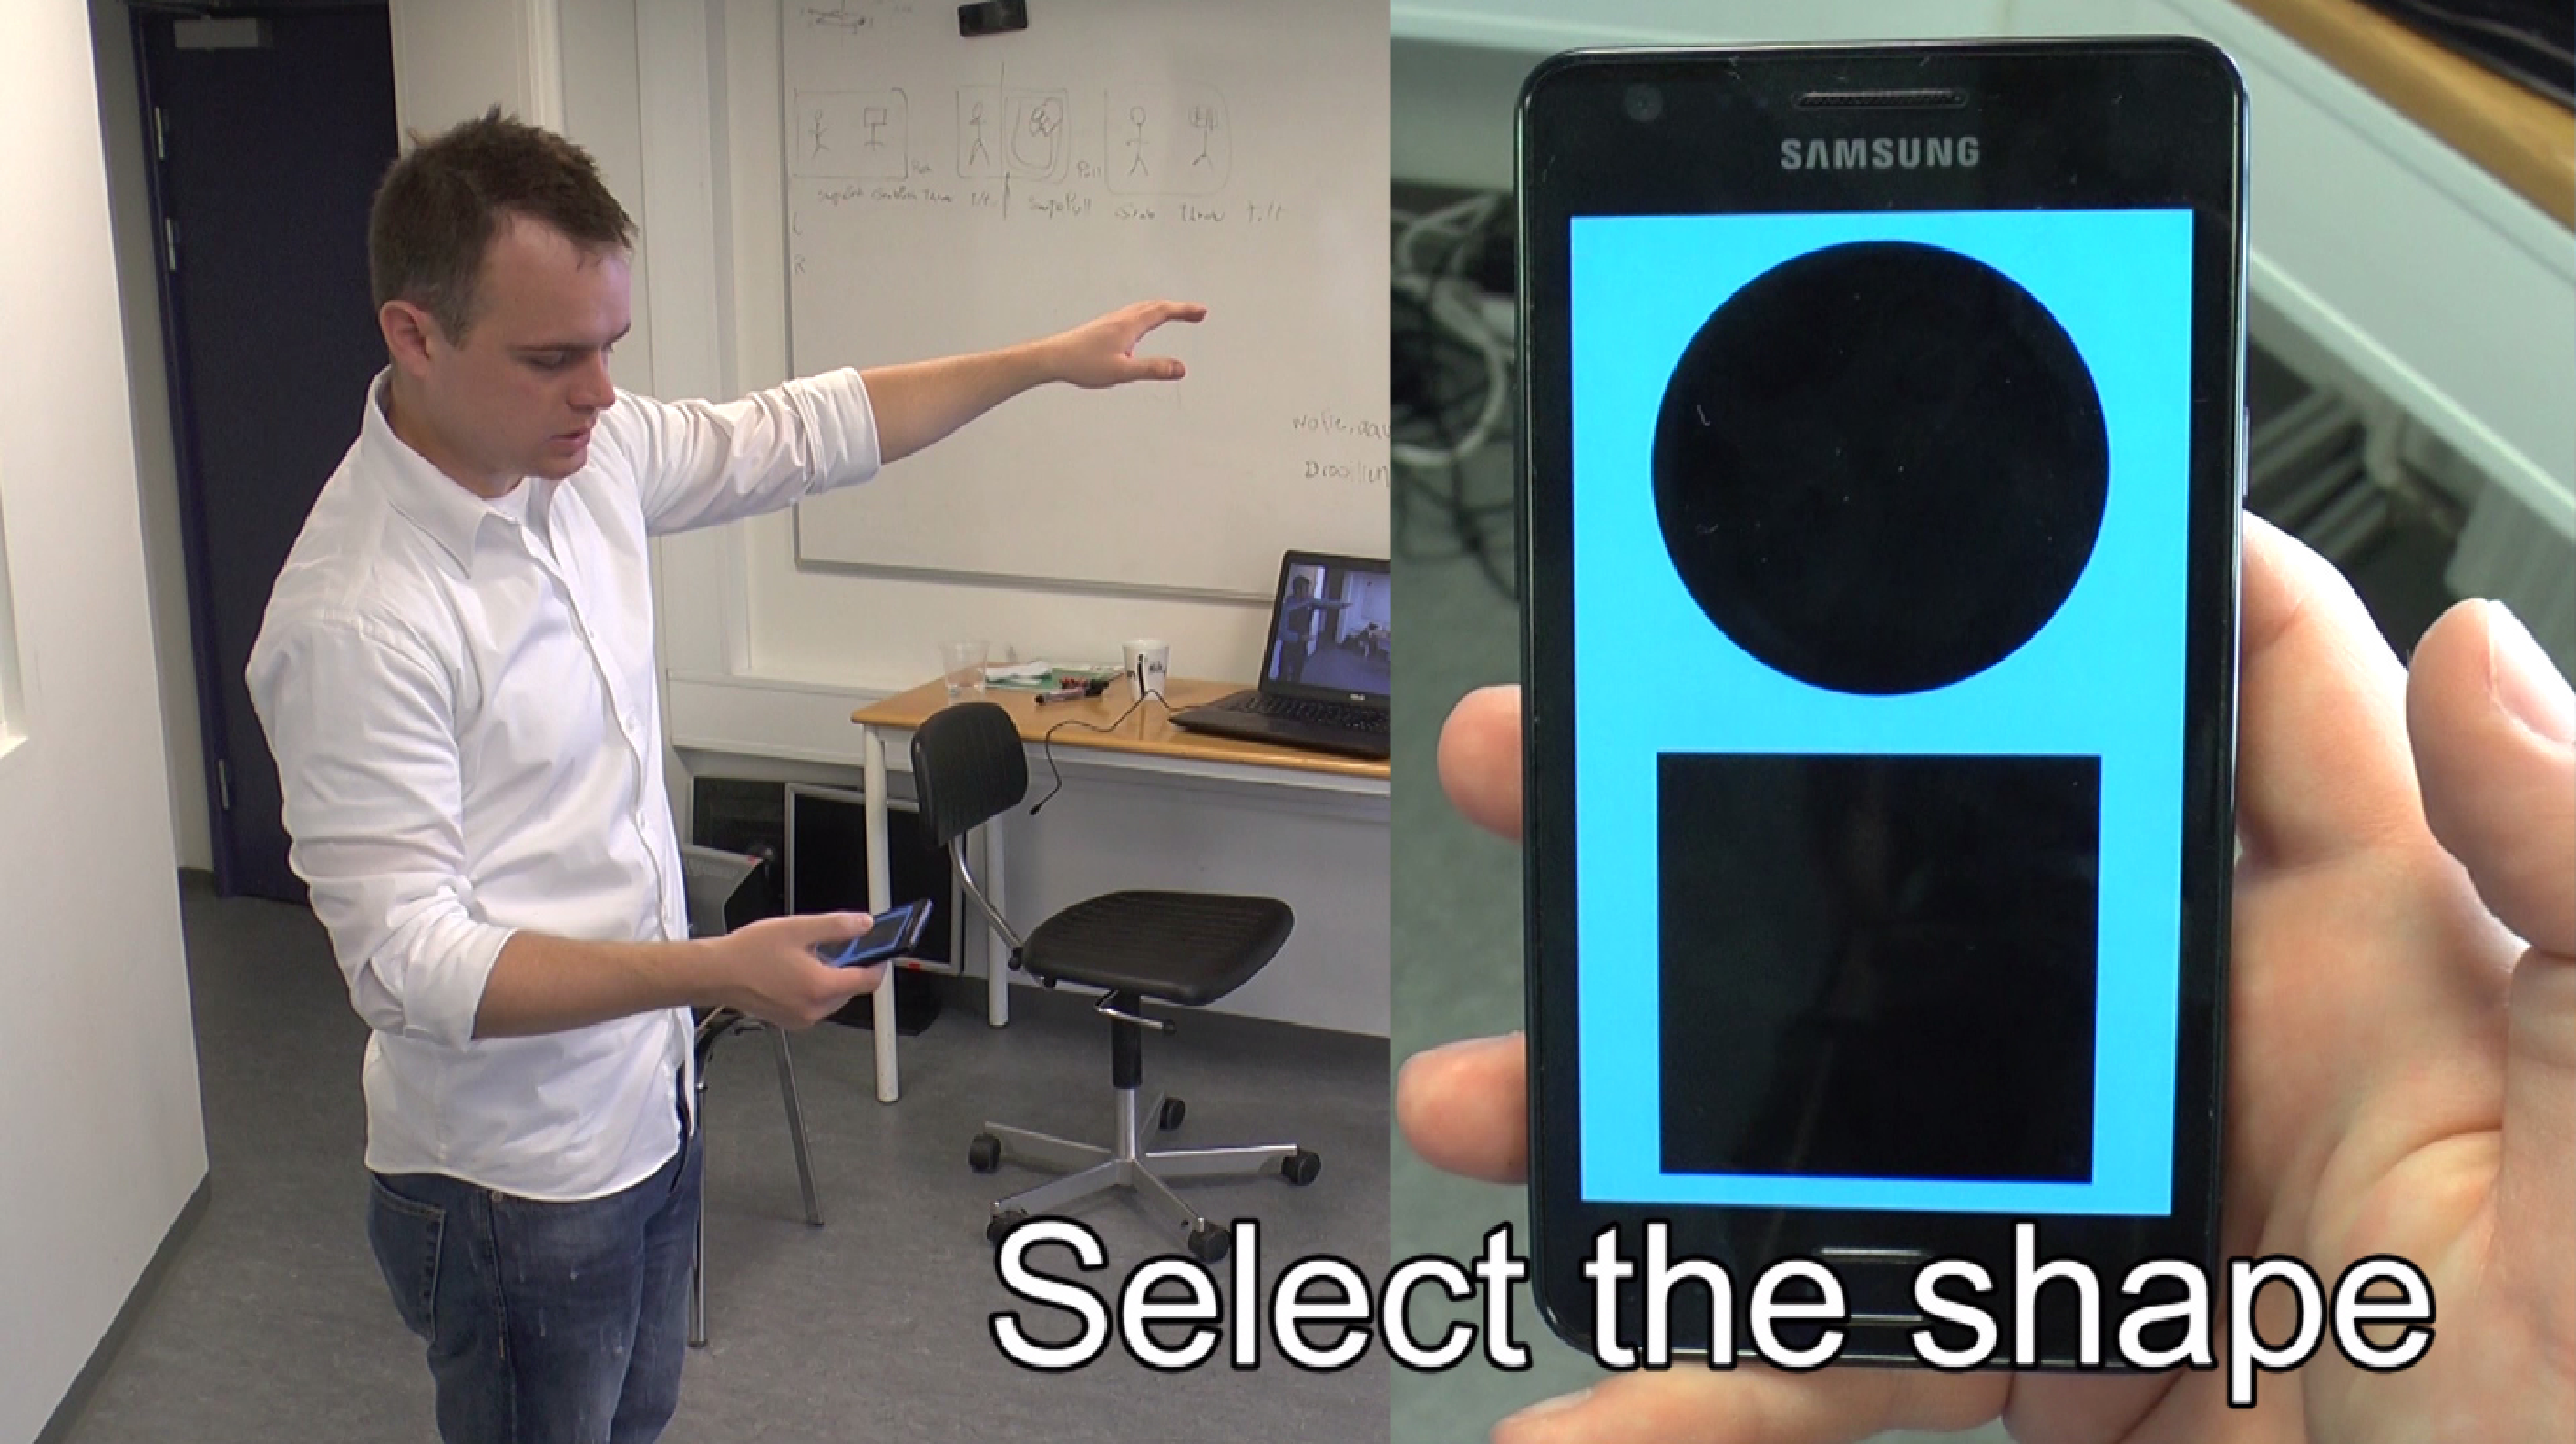
\includegraphics[width = 0.5\columnwidth]{images/demovideo3.pdf}\label{fig:demovideC}}
\subfloat[]{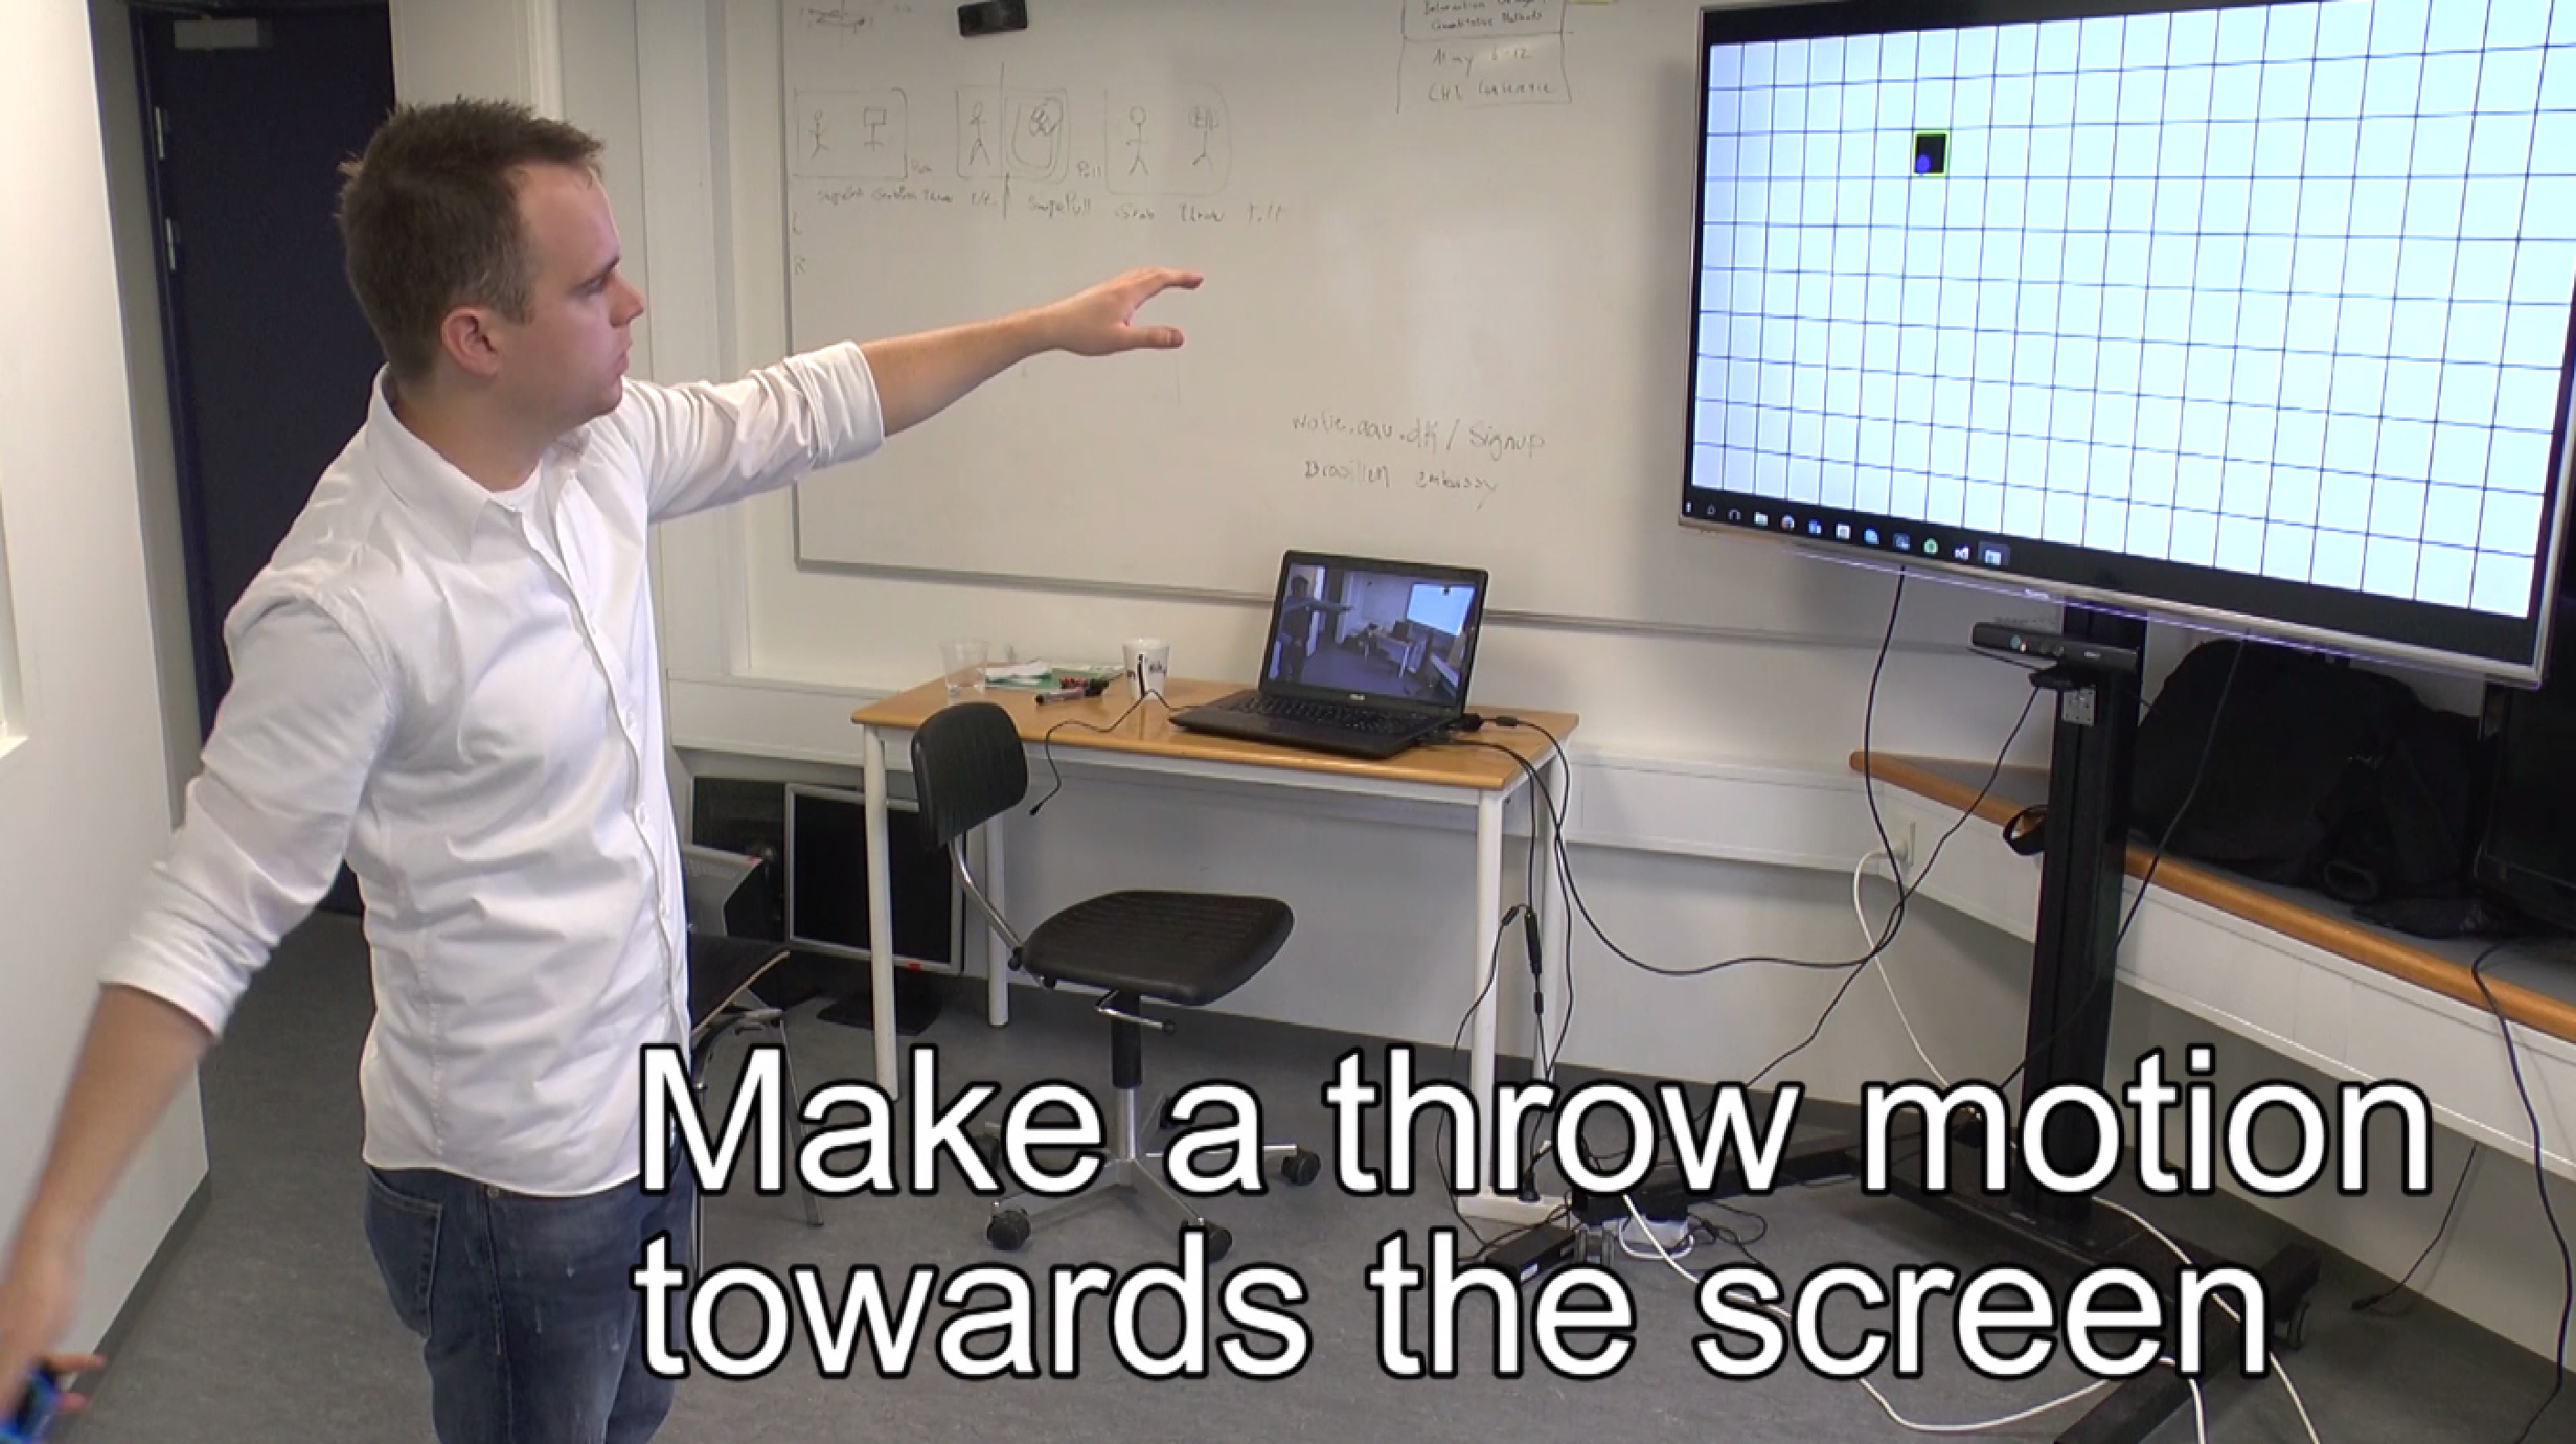
\includegraphics[width = 0.5\columnwidth]{images/demovideo4.pdf}\label{fig:demovideD}}
\caption{The screen at different times during the demonstration video. The video was shown to the participant before each technique test starts. \protect\subref{fig:demovideA} Presenting the technique with the direction and the name. \protect\subref{fig:demovideB}, \protect\subref{fig:demovideC}, \protect\subref{fig:demovideD} The video pauses and the participant will be able to read the instructions on the screen.}
\label{fig:demovideo}
\end{figure}